\documentclass[a4paper,12pt]{article}

\usepackage[utf8]{inputenc}
\usepackage[T1]{fontenc}
\usepackage{a4}
\usepackage{lipsum}
\usepackage{graphicx}
\usepackage{float}
\usepackage{listings}
\usepackage{color}
\usepackage{hyperref}
\usepackage{cite}
\usepackage{textgreek}
\usepackage{amsfonts}
\usepackage{amsmath}

\usepackage[margin=1in]{geometry}

\definecolor{dkgreen}{rgb}{0,0.6,0}
\definecolor{gray}{rgb}{0.5,0.5,0.5}
\definecolor{mauve}{rgb}{0.58,0,0.82}

\lstset{frame=tb,
  language=matlab,
  aboveskip=5mm,
  belowskip=5mm,
  showstringspaces=false,
  columns=flexible,
  basicstyle={\small\ttfamily},
  numberstyle=\tiny\color{gray},
  keywordstyle=\color{blue},
  commentstyle=\color{dkgreen},
  stringstyle=\color{mauve},
  breaklines=true,
  breakatwhitespace=true,
  tabsize=2
}

\title{
  {\Huge \bf Power Systems Lab}\\
  \vspace{0.25in}

  {\bf Experiment 3}\\
  Laboratory Report
  \vspace{1in}
}
\author{
  \bf Syed Alisamar Husain, 17BEE012\\
  B.Tech Electrical Engg, 8th Semester
}

\begin{document}
  \begin{titlepage}
    \maketitle
    \vspace*{\fill}
    \begin{center}
      {\bfseries Department of Electrical Engineering} \\
      Jamia Millia Islamia, New Delhi
    \end{center}
    \thispagestyle{empty}
  \end{titlepage}
  
  \newpage
  \begin{center}
    \huge Experiment 3
    \vspace{0.5in}
  \end{center}

  \section{Objective}
  To find the receiving end voltage, power and voltage regulation of a 
  medium length transmission line using MATLAB.

  {\bf Let the given problem be as follows:}
  \begin{center}
    \itshape
    The sending-end voltage on a 3-phase, 60 Hz, transmission line is 120 kV.\\
    The line is 100 km long and has the following constants,\\
    Impedance (Z) =  0.017 + j 0.12 $\Omega$ per km\\
    Admittance (Y) = j 1.2 $\times 10^{-6}$ $S$ per km\\
    Find the receiving end voltage and power if the line is delivering a 
    load of 17.12 MVA. Also find the voltage regulation.
  \end{center}

  \section{Theoretical Background}
  The transmission matrix, i.e. the ABCD parameters, of the line relate the
  sending end voltage and current to the receiving end voltage and current, according
  to the following equation:

    \begin{center}
      \begin{math}
        \begin{bmatrix}
          V_S \\ I_S
        \end{bmatrix}
        =
        \begin{bmatrix}
          A & B \\
          C & D 
        \end{bmatrix}
        \begin{bmatrix}
          V_R \\ I_R
        \end{bmatrix}
      \end{math}

      \vspace{12pt}      
      \begin{math}
        \begin{bmatrix}
          V_R \\ I_R
        \end{bmatrix}
        =
        \begin{bmatrix}
          A & B \\
          C & D 
        \end{bmatrix}^{-1}
        \begin{bmatrix}
          V_S \\ I_S
        \end{bmatrix}
      \end{math}
    \end{center}

  To find the receiving end power, we can simply use the following:

    \begin{center}
      \begin{math}
        S_R = V_R I_R
      \end{math}
    \end{center}

    \subsection*{Voltage Regulation}
    {\bf Voltage regulation} is a measure of change in the voltage magnitude 
    between the sending and receiving end of a component. 
    It is commonly used in power engineering to describe the percentage 
    voltage difference between no load and full load voltages distribution 
    lines, transmission lines, and transformers.

    The voltage regulation can be calculated as follows:

      \begin{center}
        \% Regulation = $ \dfrac{|V_S| - |V_R|}{|V_R|} * 100 $
      \end{center}

  \section{Implementation}
  \begin{lstlisting}
    % Receiving end voltage, power and voltage regulation of
    % 3-phase medium transmission line.

    % 17BEE012 - Alisamar Husain

    Vs = 120;     % Sending voltage in kV
    Ss = 17.12;   % Sending power in MVA

    Zp  = 0.017 + 0.12i; % Impedance per km
    Yp  = 1.2e-6i;       % Admittance per km
    len = 100;           % Length in km

    % ABCD Parameters
    Z = len * Zp;
    Y = len * Yp;

    A = ((Y*Z)/2) + 1;
    B = Z;
    C = Y*(((Y*Z)/4) + 1);
    D = A;

    T = [ A B; C D; ]
    T = inv(T);

    % Calculating sending end voltage and power

    Is = Ss / Vs;           % Sending current

    Rc = T \ [Vs;Is];
    Vr = Rc(1)              % Received voltage
    Ir = Rc(2);             % Received current

    Sr = abs(Vr * Ir)       % Received power in MVA

    % Calculating voltage regulation

    R = ((Vs - abs(Vr))/abs(Vr)) * 100 % Voltage regulation
  \end{lstlisting}

  \pagebreak
  \section{Observations}
  \begin{figure}[H]
    \centering
    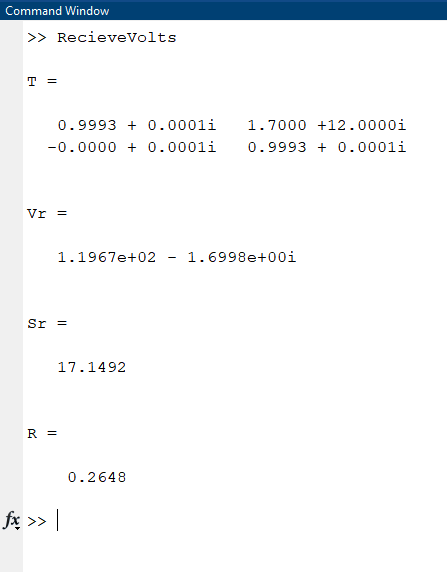
\includegraphics{img/run.png}
    \caption{Result in MATLAB}
    \label{result}
  \end{figure}
  The result of the above program with the given parameters 
  is shown in figure \ref{result}.

  \section{Result}
  For the given problem, the calculated {\bf receiving end voltage is 119.6831 kV.}
  The {\bf receiving end power is 17.1492 MVA,} which means a power loss of 29.2 KVA 
  and a voltage drop of 1.7313 kV over the line.

  The calculated {\bf voltage regulation of the transmission line is 0.2648\%.}

  Thus we calculated the requied quantities using a program in MATLAB.

\end{document}